\documentclass[twocolumn,a4paper]{article}

\usepackage{cite}
\usepackage{graphicx}
\usepackage{url}

% Bloomin' LaTex magic :o( Thanks to 
% http://iris.usc.edu/Information/ieee/latex.html

\pagestyle{empty}
        \oddsidemargin  0.5cm
        \textwidth      15cm
        \topmargin      0.0cm
        \headheight     0.0cm
        \textheight     23cm
%I copied stuff out of art10.sty and modified them to 
%   conform to IEEE format
\makeatletter
%as Latex considers descenders in its calculation of 
%   interline spacing,
%to get 12 point spacing for normalsize text, must set it 
%   to 10 points 
\def\@normalsize{\@setsize\normalsize{10pt}\xpt\@xpt
\abovedisplayskip 10pt plus2pt minus5pt\belowdisplayskip 
\abovedisplayskip \abovedisplayshortskip \z@ 
plus3pt\belowdisplayshortskip 6pt plus3pt 
minus3pt\let\@listi\@listI}
%need an 11 pt font size for subsection and abstract 
%   headings 
\def\subsize{\@setsize\subsize{12pt}\xipt\@xipt}
%make section titles bold and 12 point, 2 blank lines 
%   before, 1 after 
\def\section{\@startsection {section}{1}{\z@}{1.0ex plus 
1ex minus .2ex}{.2ex plus .2ex}{\large\bf}}
%make subsection titles bold and 11 point, 1 blank line 
%   before, 1 after 
\def\subsection{\@startsection {subsection}{2}{\z@}{.2ex 
plus 1ex} {.2ex plus .2ex}{\subsize\bf}}
\makeatother

% Different font in captions
\newcommand{\mycaption}[1]{\caption{\small{#1}}} 


\begin{document}

\twocolumn[
    \centerline{\LARGE \bf The CMS PhEDEx System: a Novel Approach to}
    \centerline{\LARGE \bf Robust Grid Data Management}
    \medskip
    \centerline{\textbf{Tim Barrass}, Dave Newbold}
    \centerline{University of Bristol, UK}
    \medskip
    \centerline{Lassi Tuura}
    \centerline{Northeastern University, USA}
    \bigskip

    \begin{@twocolumnfalse}
    \centerline{
    \parbox{13cm}{The CMS experiment has taken a novel approach to Grid data management. Instead of having a central processing component making global decisions on replica allocation, CMS has a data management layer composed of a series of collaborating agents; the agents are persistent, stateless processes which manage specific parts of replication operations at each site in the distribution network. The agents communicate asynchronously through a blackboard architecture; as a result the system is robust in the face of many local failures. CMS' data distribution network is represented in a similar fashion to the internet. This means that the management of multi-hop transfers at dataset level is simple. This system allows CMS to seamlessly bridge the gap between traditional HEP ``waterfall" type data distribution, and more dynamic Grid data distribution. Using this system CMS is able to reach transfer rates of 500Mbps, and sustain transfers for long periods in tape-to-tape transfers. The system has been used to manage branches of large scale Service Challenges for LCG this year.}
    }
    \bigskip
    \end{@twocolumnfalse}
]

\section{Introduction}
% no \PARstart
Historically High Energy Physics (HEP) experiments have been able to rely on manpower-intensive mechanisms for distributing data to geographically dispersed collaborators. The new era of CERN Large Hadron Collider (LHC) \cite{lcg:website} computing necessitates a move to more scalable data distribution and management systems; many experiments have identified Grid computing as a suitable basis for creating such systems.

CMS \cite{cms:tdr}- one of the four LHC experiments currently being built at CERN- has made important progress toward using a functioning datagrid by developing a robust data management layer. This data management layer has a simple twofold goal: to manage the prioritized transfer of files from multiple sources to multiple sinks; and to provide answers to questions of transfer latency and speedto enable scheduling of transfer operations. It bridges the gap between ``traditional" HEP data distribution- large scale scheduled transfers between major sites- and more recent grid data distribution, which enables optimized replications in response to user demand.

The data management layer, named PhEDEx, for Physics Experiment Data Export \cite{phedex:website}, is composed of a series of autonomous, robust, persistent, stateless processes. We term these processes agents, as their design is inspired by agent frameworks \cite{fipa:website,jade:website,shafi:diamonds}. These agents share information about replica and transfer state through a blackboard architecture \cite{corkhill:blackboards}. The blackboard also hosts some higher-level information about network routing, dataset subscriptions and other infrastructural information.

PhEDEx accommodates a not-completely connected distribution network- for example the tiered, hierarchical structure common to many HEP experiments. Existing Grid middleware has tended to view such structures as completely connected, and all transfers as simply single file point-to-point \cite{edg:website,guy:replicas}. More recent iterations of these applications promise to bring about great improvements in the reliability of bulk data transfers \cite{glite:website} by taking the design of PhEDEx as their starting point.

A better representation of the HEP environment is a somewhat static core infrastructure in which transfers are continuous, sourced from a central site through successive ``tiers" of sites, hosting resources of decreasing capacity. CMS will use this core infrastructure to store multiple remote, secure tape copies of invaluable experimental data in real time, relying on the core infrastructure's more robust and available services. Services capable of meeting the requirements of this task are only available at the experimental centre, and at around 10 large, geographically distributed regional centres.

\begin{figure}
\centering
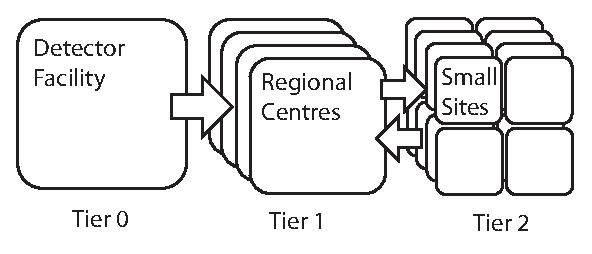
\includegraphics[width=7cm]{tiered-data-flow.eps}
\mycaption{Schematic representation of the tiered data flow common to many HEP experiments. Raw and reconstructed detector data is produced at the detector facility and flows to regional centres, where it is safely stored, and large scale analyses are undertaken. Further processed data is transferred to smaller sites for smaller scale analyses; in addition, smaller sites produce simulated data of use to the whole collaboration which is cached at the regional centres.}
\end{figure}

Smaller persistent sites that are part of the core experiment infrastructure associate with the regional centres, just as the regional centres associate with the experimental centre. By associating sites in this way the load- in terms of resource access and network bandwidth- on the experimental centre is reduced. These smaller sites take part in more dynamic tasks, like the production of detector simulation data, or analysis of data already processed at the experimental centre.

The LHC computing era brings access to a dynamic infrastructure of sites that become part of a more dynamic Grid of resources. These smaller sites typically make resources available on something close to a best-effort basis- the extreme example being a physicist�s laptop. These resources are intended for rapidly changing analysis tasks, typically with much fewer resources (storage and bandwidth). This dynamic environment is more ideally suited to management by a grid that optimizes the storage and availability of data, and is driven by end-user analysis tasks.

The key problem is to seamlessly blend very high priority, continuous large-scale data transfers between highly available resources, with smaller scale, lower priority transfers between smaller sites for analysis, re-processing or re-analysis, and therefore make the infrastructure manageable by a small number of people. The data management layer needs to do this in an environment in which even the relatively static, stable core infrastructure is considered unreliable- and must therefore handle failover and retry of transfers to a given destination. It is also conceivable that high-priority transfers might get dynamically reallocated in the face of failure of a regional centre, guided by collaboration policy. 

The data management layer should provide sufficient functionality to allow a person or process to specify some group of files and a number of destinations, and then have the layer manage the efficient replication of data from wherever it currently resides to those destinations. The data management layer should also be capable of harvesting data from creative processes, introducing that new data to

By devising a system in this manner, we meet the immediate needs of HEP experiments- which are typically the traditional large-scale directed transfers- by plugging in a simple replica management algorithm that takes subscriptions for datasets, and manages transfers as they become possible, without having a manager oversee the entire transfer process. We also make it possible to add to this simple replica management a more sophisticated optimizing replica manager as the system matures.

\section{Overall use cases for HEP data distribution}
In HEP there are two broad use cases for a data management layer: ``push" and ``stream" (or ``pull"). Push indicates the transfer of invaluable raw experimental data from the detector to tape store at regional centres. In this case, the collaboration chooses which regional centres store which data, and pushes the data onto them. It is this use case that is the source of the differences between PhEDEx and existing file distribution systems. To operate efficiently it must be possible to clear newly-created files in buffer space at data sources; to do this it is vital to know whether that file has been made ``safe", where ``safe" is defined as ``in tape storage at the detector facility and at least one regional centre". To do this PhEDEx maintains monitors the transfer and migration of files, and is given responsibility for cleaning buffer space when it knows that files are safe at their destinations.

The streaming use case represents another on-going process instigated by either a regional centre, or a relatively stable smaller site. In this case, the site can subscribe to a given dataset; as files in this dataset are created, wherever they are created in the distribution infrastructure, they are transferred to the subscribing site. Similarly, these sites must make the data they create available for streaming to other sites.

The pull use case is a subset of stream, and represents a small-scale one-shot operation, in which say a single physicist is interested in some part of a dataset, and wishes to transfer it either to their University or even their laptop. In this case the end user would just connect their laptop or other resource to the data management layer, specify the data required, wait for the data management layer to transfer the necessary files and then remove the laptop from the layer.

Note that the names of these use cases are not intended to describe low-level transfer activity. In all cases we implement point to point transfers as third party- although in the majority of cases they are instigated by an agent running near the destination rather than the source.

The simplest requirements placed on the system are that it should be manageable at a high level by an individual, and that low level deployment and support take close to zero effort. To meet these requirements we devised an architecture based on quite simple, focused, robust processes that were able to handle failover and retry of transfers autonomously, and which could collaborate to solve the problem of transferring data over multiple hops to multiple destinations.

FIXME: Performance requirements ...

The system should also scale by the number of files in transfer. It should have a robust, internet-like design where no one part can bring entire transfer network down. The system should be able to saturate any hardware (network, storage) on which it is deployed. It should also operate completely asynchronously from other systems, for example: data management systems; data production processes; or analysis tasks running on batch computing nodes.

Within PhEDEx we have met, or will soon meet many of these requirements.

Note that what we do not discuss here is co-scheduling of replication with jobs. In this environment the cost of replication is very much higher than the cost of running a job, and therefore it makes sense to distribute data throughout the collaboration and then send jobs to the data.


\section{Comparison with other replication technologies}
The scale of data distribution for the LHC experimentsis therefore much larger than previous experiments....

There have been many advances in replication technology in recent years, with the development of data Grids and peer to peer filesharing technologies...

\subsection{Previous methods for distributing HEP data}
Existing HEP experiments tend to manage data distribution in a structured but manpower intensive ways. One such example is the use of rsync to manage the periodic transfer of data files from an authoratative source to a remote site. This was typically done by issuing commands whenever a tranfer was required, rather than by having an automated process manage the transfers. This was the approach taken by, for example, the BaBar experiment \cite{babar:website}. More recently the BaBar experiment has investigated the use of the Storage Resource Broker to distribute and manage access to it's data \cite{babar:srb}; it also has a home grown application named BdbServer++ that enables users to locate distributed replicas and create a complete dataset replica on the user's laptop \cite{babar:distribution}.

For job data management the D0 \cite{d0:website} and CDF \cite{cdf:website} experiments use a sophisticated system named SAM \cite{sam:website} which couples every aspect of data gathering and access together. Data replication and tape management, however, is still a complicated manual operation, even when using this system. In both cases these solutions are ideal, as data is not distributed to a large number of sites, and the solutions therefore scale adequately.

\subsection{Grid Computing Technologies}
Most Grid technologies are focused on the running of jobs rather than on the large scale replication of data; the latter is currently a larger problem for HEP experiments.

For example, Condor \cite{condor:website} and its Grid-equivalent, Condor-G, focus very much on the running of jobs, and views the management of data to be something to be solved by external processes. Similarly, commercial products and services like the Sun Grid Engine \cite{sungrid:website} focus on providing the resources to run jobs rather than managing the replication and custody of data over a number of distributed sites.

A large scale EU project named the European DataGrid (EDG) \cite{edg:website} was initiated to develop a Grid infrastructure that would meet the needs of HEP, Biology and Medical Imaging, and Earth Observation research to access significant distributed computing resources. The project- now replaced by EGEE (Enabling Grids for ESciencE) \cite{glite:website}- developed a number of low-level infrastructural elements that can be used to build a data Grid. However, the components assume a completely-connected network of peers; data replication was intended to be undertaken in response to demand, rather than policy; and there was no sense of custody or responsibility for data outside of a source site.

\subsection{Peer-to-Peer Filesharing}
A number of peer-to-peer filesharing applications have appeared since the origin of Napster in 1999. They vary in nature between more-centralized systems in which peers and replicas of data are tracked in a manner similar to instant messaging systems, and less centralized in  which client communication is more truly peer-to-peer and doesn't rely on centralized services to make contact with peers or find replicas. An example of the former is BitTorrent \cite{bittorrent:website}, and of the latter, GnuTella \cite{gnutella:website}.

One important benefit of peer-to-peer filesharing is the ability to download a file from multiple sources: the file is split into blocks, and the client replicates blocks from whichever peers are capable of serving them. This concept is easy to map onto HEP data without developing mechanisms for splitting files, as HEP data is typically organised into datasets which form the basic unit of access; therefore the basic unit of distribution in HEP is the dataset rather than the file.

There are however differences between the environment managed by existing peer-to-peer applications and the HEP environment. Typically peer-to-peer systems assume a completely transient, dynamic environment in which most routes are short-lived. To avoid network segmentation in this environment existing peer-to-peer apps create random peer topologies to minimize the consequences of peers losing contact. In contrast, the HEP environment is characterised by well-funded and managed dedicated high-speed links between large international institutions that are relatively long lived. HEP distribution topologies are therefore more structured as the links between peers are maintained by social contract rather than by transient applications.

Furthermore, existing peer-to-peer systems have no sense of the value of data, or any sense of custody of data at sites remote to the original source. P2P clients are typically characterised by on-demand transactions rather than the continuous sustained replications that characterise the bulk of HEP distribution.

Note however that in addition to these core activities HEP experiments need to maintain the flexibility to enable typically chaotic analysis activities, and to meet sudden demand for specific ``hot" data, and this is where Grid computing and peer-to-peer services are of most use. In general though no technology completely meets HEP experiments' needs for managing secure custody of data and maintained large-scale data transfers; hence the CMS experiment decided to develop PhEDEx.

\section{Current PhEDEx architecture}
\subsection{Introduction}
HEP environments are typically heterogeneous at all levels of operation, although some standards in transfer tools and storage management are beginning to emerge. To develop PhEDEx we rely on a core set of tools and services that are most widely available. These tools and services are broadly cataegorized as either storage management or transfer tools.

For storage management we rely on SRM (Storage Resource Management) \cite{srm:website}, which provides generic access to any storage resource. Superficially SRM provides a defined two step interaction through which a file can be obtained from any storage resource by using a Storage URL (SURL), which contains the hostname of the resource and some identifier that can be interpreted by the resource. During an SRM transaction the client presents an SRM server with the SURL; the server returns a Transport URL (TURL) which indicates the current (possibly temporary) location of the file and a transport protocol that can be used to access it. This means that someone wishing to access a file at a given site does not need to know on which or what type of physical resource the file resides. 

In conjunction with SRM, local file catalogues map some (collaboration level) global replica set identifer to some (local) identifer that can be used to access the file. These catalogues are not strictly seen as part of PhEDEx, as they are shared with other activities at each site- analysis tasks, for example. In this context ``catalogue" is quite a generic term: it could refer simply to the internal catalogue maintained by the filesystem, or to something more complex like a MySQL database that serves file information for multiple tasks, including distribution.

A number of tools are used for point-to-point transfer of data. WAN transfers are made with tools that overlie GridFTP \cite{gridftp:website}- basically FTP with X509 certificate authentication. Such tools are globus-url-copy \cite{globus:website} and srmcp \cite{srm:website}. PhEDEx also uses a number of site-local transfer and tape management commands. This variety of tools is accomodated with a plug-in design that allows the system to provide generic components that can be easily configured to use local tools when necessary.

\subsection{System design}
PhEDEx design and development is guided by a number of architectural principles. The key principle is that complex functionality should be kept in discrete units, and that the handover of responsibility for sections of the transfer workflow should be handed between those units using as few messages- containing minimal information- as possible \cite{bryson:complexity}. As the system comprises active components it is reasonable to model these units after agents rather than as passive stateless services.

The PhEDEx design is characterised by layered abstractions. Our experience with data management tools has led us to view many operations and tools as unreliable. To manage this we wrap unreliable tools and systems in more robust layers to build a reliable data transport system.

\begin{figure}
\centering
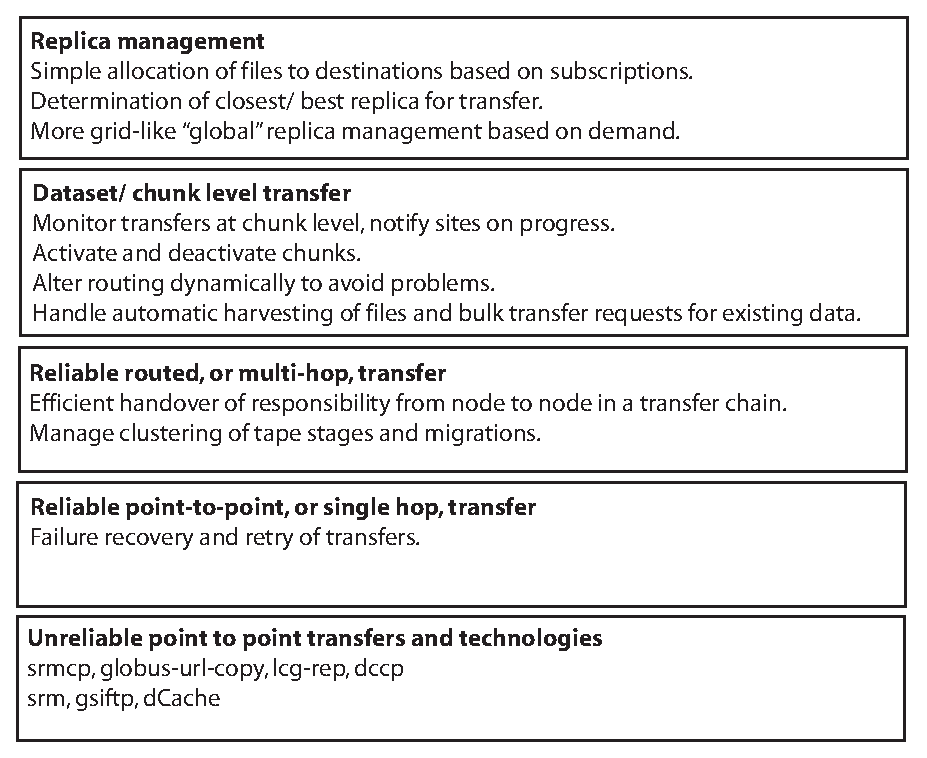
\includegraphics[width=7cm]{phedex-layers.eps}
\mycaption{PhEDEx' layered architecture. Each layer is considered more reliable than the one below. For example: transfer tools are considered unreliable due to- in many cases- lack of reasonable failure recovery and unreliable error returns. The tools are therefore overlain by a layer that handles pre- and post-transfer validation checks and the subsequent retry of failed transfers. This layer also handles the collaboration between agents required to manage the clustered request and stage of data from tape, among other functions. }
\end{figure}

In addition, PhEDEx allows site managers to keep local information local, and allow as much local management of files as possible. This makes the system robust during local infrastructural change, but means that local and global information can become unsynchronised after deletion operations. For example, moving files from one local disk to another is transparent if local catalogues are also kept up to date. However, file deletion requires an update of the PhEDEx system. This is not considered unscalable, as the straightforward deletion of files is rare in HEP systems: although data can be invalidated, it is rarely deleted. More problematic is the loss of files due to hardware failure; in this case PhEDEx currently relies on close interaction with local admin so that such failures are quickly accomodated.

To guide development we avoid creating services that aren't necessary, generally by accepting a small increase in complexity on the ``client" transfer components. To make message passing simple we utilise a blackboard architecture in which transfer components post state information. The blackboard is currently deployed as a single high availability database. We also leverage data chunking to improve performance by avoiding somewhat traditional file-to-site mappings, instead mapping files to chunks and chunks to sites; we don't, however, require a chunk to exist anywhere in entirety.

\subsection{Overview of transfer operations}
The core element of the data management system is a node- a logical entity to which persistent processes named agents are associated. Typical examples might be a regional centre's transfer node, with agents to, for example, manage transfers from the centre's neighbours to the centre's disk buffers; or a mass storage node with an agent to manage the clustering of requests from other nodes for files for transfer.

Transfer workflows are divided into functionally coherent units- file transfer, for example, or migration to tape. Within those units workflow stages are defined as internal state transitions.  The handover of responsibility for a replication between units are seen as messages passed between agents, and are currently represented as state transitions on the blackboard. By way of example, the state transitions of a file transfer are: predelete, transfer, verify, postdelete, publish catalogue. The messages passed between agents involved in the transfer of files are for operations like: marking a number of files as wanted; or as being ready for transfer or migrate. This message passing represents the collaboration of agents to achieve their goals.

\begin{table*}
\renewcommand{\arraystretch}{1.3}
\mycaption{Broad agent functionalities}
\centering
\begin{tabular}{p{3cm}|p{10cm}}
\hline
\bfseries Agent type & \bfseries Description \\
\hline
\hline
Allocator & Allocates blocks of files to destination based on subscriptions and collaboration policy \\
Download & Manages the point to point transfer of files \\
Export & Manages the process of making files available on request by a Download agent \\
FileRouter & Triggers transfer hops for a given node based on nearest replica algorithm \\
NodeRouter & Maintains a node's routing table and contact with neighbours \\
Stager & Manages the bulk staging of files from tape to disk \\
Migrator & Manages the migration of files to tape \\
Cleaner &  Removes stale or unrequired replicas from disk \\
\hline
\end{tabular}
\end{table*}

\begin{figure}
\centering
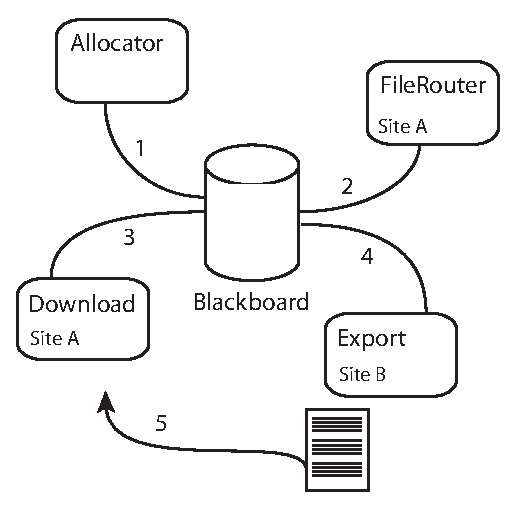
\includegraphics[width=7cm]{sample-workflow.eps}
\mycaption{A sample exchange between agents to manage the replication of a file. 1: Allocator agent recognises that new files are available at site B for transfer. Using subscription information it allocates those files to a set of final destinations- in this case site A. 2: FileRouter agent working at A finds the new file allocated to it, finds a replica at B and posts a B-A transfer request. 3: Download agent at A selects a group of files for transfer and marks them as ``wanted" 4: Export agent at B clusters the wanted files from all its neighbours and requests their stage in a manner that is efficient for local resources. When they are staged it marks the files as ``available". 5: Download agent uses some transfer tool to replicate available files. It then validates the transfer, publishes the file to a local catalogue and marks the transfer as complete.  }
\end{figure}

The blackboard space that agents use to exchange messages/state information was envisaged as a database schema. This database schema provides us with a structure for defining a set of message ontologies, and its deployment as a database provides us with a reliable mechanism of communication. The information stored in this schema tracks the list of files currently of interest to the data management system, useful metadata concerning the nodes in the system (names, routing information) and high level subscription information (which sites subscribe to which datasets, and which files are currently allocated to which specific node). It also tracks the current state of point-to-point transfers, and maintains an index structure that maps global replica set identifiers to nodes in the distribution network.

Note that the database schema is designed with the goal of insulating information that is considered ``local": all tables are logically partitioned by node where possible, and agents typically only touch data concerning their own node, or that of their neighbours.

Agents are defined at a high level only, in terms of their functional behaviour and expected interactions with other agents. They are developed using an agent toolkit, which wraps much of the low level functionality in common to all the agents: for example, handling database connections in a robust manner, or processing job queues. An explicit decision was made at the start of the project to wrap core message passing/ database access in a toolkit rather than to provide services that overlay the databases. 

The advantage of making agent code simpler through the deployment of services to handle chunks of complex functionality was deemed lower priority than the minimisation of maintenance and support effort required to maintain a performant service- especially when robust services to handle database interactions already exist: for example Oracle and MySQL both provide services to allow remote database interaction- to a large extent there is no need to create a new service over the top, however thin. This approach was taken in interactions with both the blackboard and, where possible, local file catalogues.

%\section{Specific operations}

%\subsection{Injection of files into distribution}

%\subsection{File routing}
%Possible routes through the network are represented by routing s in the central blackboard database. The routes in these routing tables represent a high-level network that overlays the internet (such networks are named overlay networks in peer-to-peer terminology). Each node in the network runs an agent which uses an implementation of the well-known RIP alogorithm to maintain links with neighbours and discover or time-out routes to other nodes in the network. Using this algorithm routes can be automatically removed from the network when the node (and its routing agent) go down.

%Files are discovered and routed through this network by a complementary set of agents that execute at and act on behalf of each destination. These file routers poll the blackboard to discover whether their node has any data allocated to it. On finding allocated data, the file routers search for replicas of that data; they determine which replicas are closest (fewest ``hops") to their node and trigger a transfer for each. Note that the routers do not actually handle transfers- they just post a state in the blackboard describing a transfer that should happen for a particular file between two particular nodes.

%This routing of replicas is currently undertaken on a bulk basis- a transfer for every existing replica for a dataset is triggered in one iteration, with no consideration for whether in time another node might be more suitable as a source. This is one area where the incorporation of established peer-to-peer filesharing strategies would be useful.

%\subsection{Transfer operations}
%PhEDEx transfers are managed with an interaction between a number of agents. Download agents acting on behalf of a node poll the blackboard to determine whether a transfer from a neighbouring node as been requested by a file router. The Download agent sorts and prioritises the currently requested transfers, and then marks some subset of the files as wanted.

%Export agents at the sites holding the desired replicas discover that some of their replicas have been marked as wanted, and make them available for transfer. This may involve staging them to disk, and posting a SURL with which to access the file on the blackboard.

%When the Download agent becomes aware that files are available for transfer it goes through the following process. First of all it determines where to place the replica it will create. It then removes any existing replica at that location; this is important to make the transfer robust, as many transfer tools create a zero size file on failure, and then fail on successive attempts to overwrite the file. The Download agent then makes a third party transfer, and verifies that the size and checksum of the transferred file are as expected. If the transfer is successful the Download agent publishes the new replica to its local catalogue and marks the transfer as complete on the blackboard.

%In this way PhEDEx gives replica-hosting nodes the opportunity to manage bulk staging of files; it also means that stagers at the replica-hosting nodes aren't overwhelmed with multiple repeated stage requests for the same files. Transfers are never started until files are staged- which means that transfers don't time out waiting for those stages.

%\subsection{Managing Buffer Space}
%Migration of replicas and marking files safe.

%Buffers are then cleaned by cleaner agents. These agents act as garbage collectors: they check with the replicas on a given node are required. Typically, if the file has reached all currently known destinations then the replicas created and cached at intermediate buffers are no longer required, and can be deleted.

\section{Scalability Tests}
By design it is easy to deploy a self-contained PhEDEx testbed in which all operations (if necessary) can be faked: for example, fake transfers (with no file movement) can be set to succeed immediately every time, or to succeed or fail with a finite time governed by a statistical analysis of real operational data. On a test network of 5 nodes- a similar number to the number of regional centres in CMS- it is possible to show that PhEDEx can replicate around 30,000 files an hour (which translates to approximately 200,000 routing decisions an hour).

In addition, PhEDEx can handle of order $10^6$ files in transfer at any given time. This performance is currently being enhanced by considering replicas of file sets rather than files, thus limiting the number of files considered at any given time.

\section{Operations}
PhEDEx is currently deployed at 8 large CMS regional centres, as well as a number of smaller sites. It manages transfers between a variety of storage resource types: SRM, gsiftp servers, dCache \cite{dcache} disk pool managers, and a variety of underlying tape storage technologies (Castor \cite{castor}, Enstore \cite{enstore}, ADS \cite{ads}). WAN transfers are managed using globus-url-copy and srmcp.

All sites are capable of downloading data; some sites are capable of uploading data. By far the largest problems encountered have been in managing problems with the underling storage and transfer technologies. Although SRM is in some sense a standard, there is sufficient variation between implementations (and versions of implementations) to mean that installation and upgrade is not trivial; differences in implementations have led to a number of problems resulting in failed transfers.

Bandwidth is very rarely an issue as the experiment doesn't have enough data to saturate current networks and hardware for extended periods of time. The stability of the underlying systems is frequently problematic, meaning that the system generally is not completely ``up" for more than a day at a time. On average about a third of the network is down, although obviously the system is able to maintain transfers in the face of these problems thanks to its design. Identifying problems is typically a very lengthy procedure, as we deal with compicated stacks of softare deployed at widely distributed sites with varying levels of support.

The majority of the agents have been developed as perl scripts that call other transfer tools. Communication with other agents through the blackboard database is via wrapped client-side SQL.

As of June 2005 PhEDEx managed over 200TB of data. In the preceding 6 months it managed the transfer 45TB of data, with some sustained transfers of nearly 20TB a month. PhEDEx proved able to manage aggregate transfer rates in excess of 500 Mbps, including PhEDEx overhead for catalogue publishing and validation of transfers. Our current experience with the system is that efficient tape staging is the key bottleneck in the system: high rates can be achieved disk-to-disk, but stage pools are rapidly depleted of files to transfer. Generally the highest real stage rates achievable for tape stages are ~300Mbps; efficient tape stages represent the most keenly-sought improvement in our performance.

\section{Future developments}

\subsection{File Routing by Contract Tender}
At present the files of a dataset are routed through the network on a bulk basis without concern for whether the node chosen at a given time might continue to be the best source for those files. A simple modification of the existing routing mechanism would be to only route subsets of a dataset at any given time, and to wait for transfers to complete before routing any more of the files. This would allow the system to take advantage of the data becaming available from a closer or more available node. A simple measure of more available in this case might be just the number of sucessfully completed transfers between two given nodes in the last hour, for example.

However, this mechanism is unlikely to be much more scalable than the existing mechanism; both make quite heavy database queries to make their routing decisions. An alternative is for a filerouter to send out a tender for transfer contracts: agents at each of the nodes where a replica for a given file exist would determine the cost of supplying that file, and hand their response over to the next hop in the transfer chain. A similar agent at the next hop would determine it's cost for supplying that files, and hand over to the next hop, and so on, until a total cost for each chain of possible transfers from replicas to destination had been established. The destination file router could then choose the lowest-cost transfer chain for each file and trigger transfers as necessary.

\subsection{Policy and Priority}
Explicit handling of "priority" at various granularities: what does priority mean, why do we need it, moving to priority based replica management (straightforward extension of simple scheduling/subscription replica management).

\subsection{Decentralization}
At present the use of a single point-of-failure database is only a theoretical problem; indeed, the central blackboard has been the most stable component of the system. Peer-to-peer filesharing applications like BitTorrent also have similar single-points-of-failure and are also demonstrably robust. There are obviously, however, arguments for decentralizing sections of the information in the central blackboard.

Routing table design is partitioned, and responsibility for a node's routing table could be easily devolved to a particular agent with its own database. However, then need agents to communicate directly with their neighbours to maintain their routing table...

The load on the central blackboard might be lessened by smearing information across nodes using a peer-to-peer alogorithm like Kademlia. A good candidate for this treatment is replica location information. Algorithms like Kademlia work by   giving each node in the network a unique identifier generated with a random hash function. Replica sets can similarly be given unique identifiers, and then information about those replica sets can be held at one or more nodes with node identifiers that are algorithmically close to the replica set identifer.

Of course, decentralisation is not without cost; in this context decentralisation makes it more difficult to determine aspects of system state. In relation to the specific mechanisms described above it would become much harder to build a complete routing table, for example, or to locate all replicas of a dataset.

\section{Conclusion}
The conclusion goes here.

\bibliographystyle{IEEEtran.bst}
\bibliography{IEEEabrv,./barrass_et_al}

\end{document}


